\documentclass[sigconf]{acmart}

\usepackage{booktabs} % For formal tables
\usepackage{enumitem}
\usepackage{balance}
\usepackage{algorithm}
\usepackage[noend]{algpseudocode}
\usepackage[labelfont={bf},aboveskip=0pt]{caption}
\usepackage[farskip=0pt,nearskip=0pt,captionskip=0pt]{subfig}
%\usepackage{underscore}
\renewcommand\_{\textunderscore\allowbreak}

\newcommand*{\TitleFont}{%
      \usefont{\encodingdefault}{\rmdefault}{b}{n}%
      \fontsize{20}{20}%
      \selectfont}

\setlength{\parskip}{0pt}
\setlength{\floatsep}{5pt}
\setlength{\dblfloatsep}{5pt}
\setlength{\textfloatsep}{5pt}
\setlength{\dbltextfloatsep}{5pt}
\setlength{\skip\footins}{7pt}

\widowpenalty=0
\clubpenalty=0
\brokenpenalty=0

\AtBeginDocument{%
 \abovedisplayskip=0pt
 \abovedisplayshortskip=0pt
 \belowdisplayskip=0pt
 \belowdisplayshortskip=0pt
 \jot=0pt
}

\linespread{1.0}

\settopmatter{printacmref=false} % Removes citation information below abstract
\renewcommand\footnotetextcopyrightpermission[1]{} % removes footnote with conference information in first column
\pagestyle{plain} % removes running headers

\begin{document}
\title{Estimate S-Wave Arrival Time, Find Hypocenter, Predict Magnitude of Earthquake with DNN}
%\title{\TitleFont Estimate S-Wave Arrival Time, Find Hypocenter, Predict Magnitude of Earthquake with DNN}

\author{Seongbeom Park}
\affiliation{Student ID : 20165112}
\email{amita90@unist.ac.kr}

\author{Jinsu Park}
\affiliation{Student ID : 20165126}
\email{jinsupark@unist.ac.kr}

\maketitle

\section{Design and Implementation}

We build a deep neural network (DNN) to estimate when the earthquake strikes to the cities (i.e., ADO, RPV, RSS and USC), find the epicenter and depth of the hypocenter, and predict magnitude of the earthquake. Figure ~\ref{fig:overview_model} show overview of the model.

\begin{figure}[t]
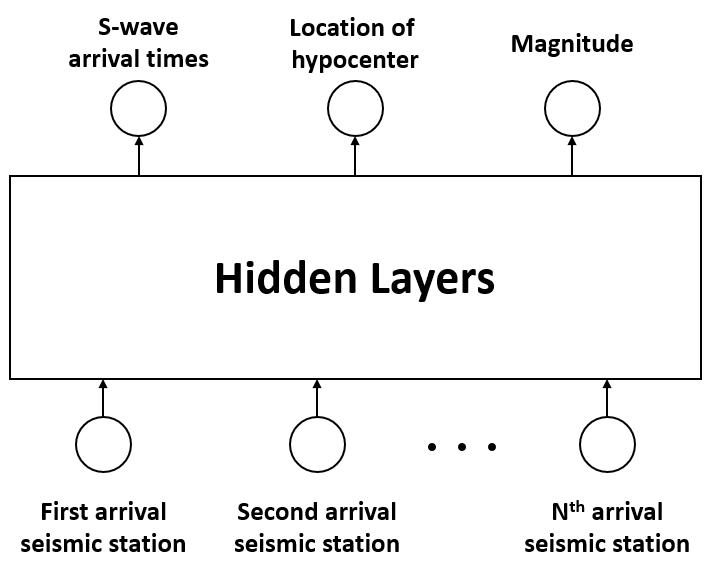
\includegraphics[width=0.48\textwidth]{figs/overview_model.png}
\caption{Overview of DNN model}
\label{fig:overview_model}
\end{figure}

The model uses input features as latitude and longitude of seismic stations and arrival times of P-wave which is encoded in various formats. We use three loss functions to train our model. It is called multitask learning \cite{baxter1995learning} which prevents overfitting problem by designing a model to estimate various related tasks at once.

The model predicts three components. First, it estimates the arrival times of S-wave for each seismic station. It uses average of absolute difference of S-wave arrival time as a loss to train the model. The model optimizes (minimizes) the loss with ADADELTA \cite{zeiler2012adadelta} optimizer.

Second, it finds the epicenter and depth of the hypocenter. It uses mean squared error of latitude, longitude and depth to calculate the loss. The function simply emulate the difference of distance between hypocenter and predicted hypocenter. The model optimizes (minimizes) the loss with ADADELTA optimizer.

Third, it predicts magnitude of the earthquake. It uses absolute difference of magnitude for the loss function. The model optimizes (minimizes) the loss with ADADELTA optimizer.


\section{Evaluation}

The dataset is devided into training dataset and test dataset. Training dataset includes 80\% (299 earthquakes) of total dataset and test dataset includes 20\% (75 earthquakes) of total dataset. We trained the model 50 steps and shuffled training dataset in each steps to prevent overfitting.

%%%

Figure ~\ref{fig:arrival_loss_10} shows the loss of S-wave arrival time with 10 fast earthquake arrived seismic stations.

\begin{figure}[t]
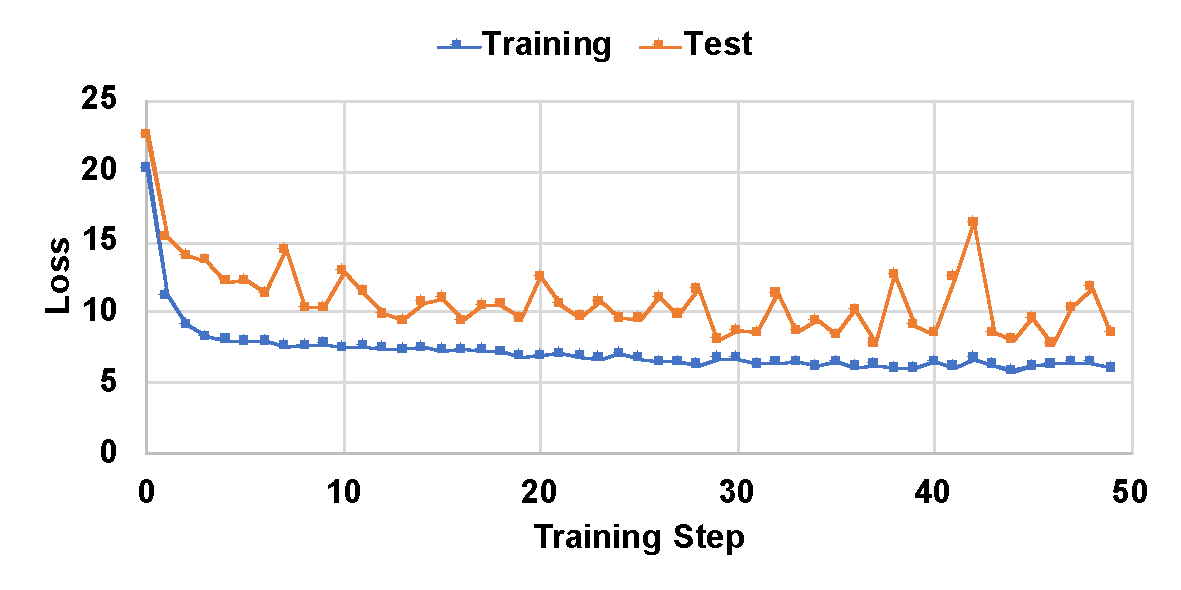
\includegraphics[width=0.48\textwidth]{figs/arrival_loss_10.pdf}
\caption{Loss of arrival time estimation with 10 seismic stations}
\label{fig:arrival_loss_10}
\end{figure}

Figure ~\ref{fig:center_loss_10} shows the loss of location of hypocenter with 10 fast earthquake arrived seismic stations.

\begin{figure}[t]
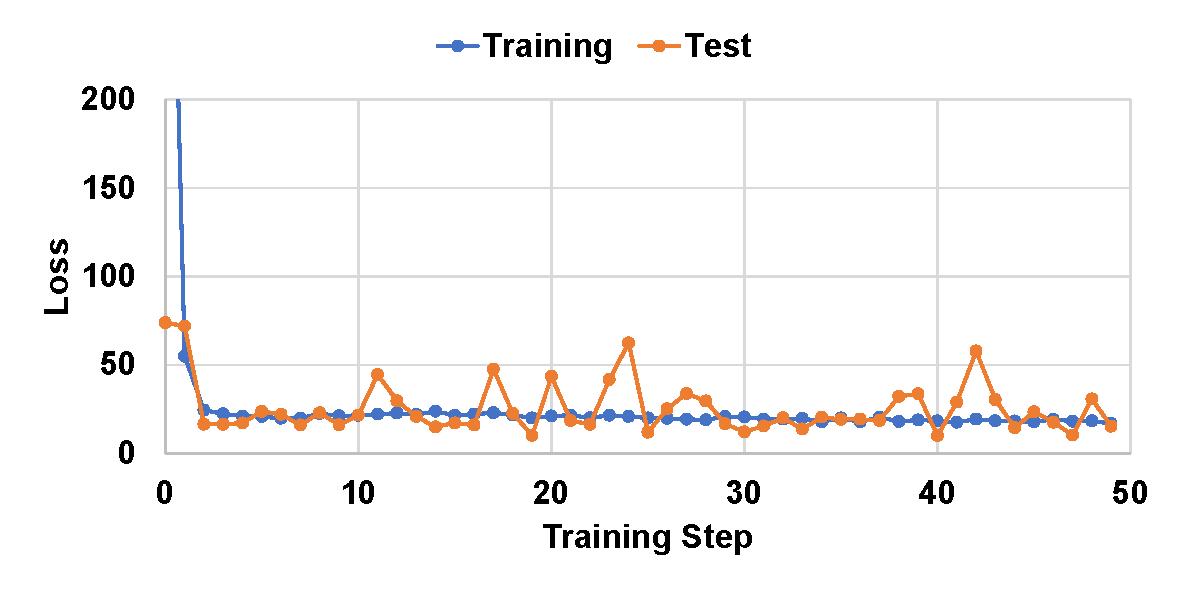
\includegraphics[width=0.48\textwidth]{figs/center_loss_10.pdf}
\caption{Loss of hypocenter estimation with 10 seismic stations}
\label{fig:center_loss_10}
\end{figure}

Figure ~\ref{fig:mag_loss_10} shows the loss of magnitude with 10 fast earthquake arrived seismic stations.

\begin{figure}[t]
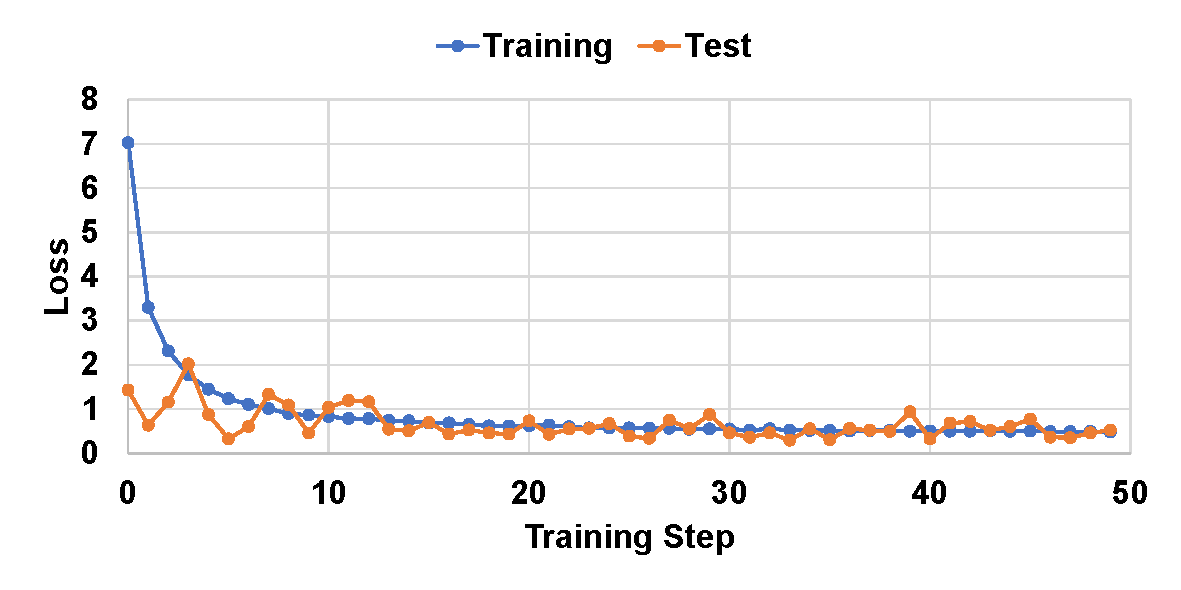
\includegraphics[width=0.48\textwidth]{figs/mag_loss_10.pdf}
\caption{Loss of magnitude prediction with 10 seismic stations}
\label{fig:mag_loss_10}
\end{figure}

%%%

Figure ~\ref{fig:center_loss_3} shows the loss of S-wave arrival time with 3 fast earthquake arrived seismic stations.

\begin{figure}[t]
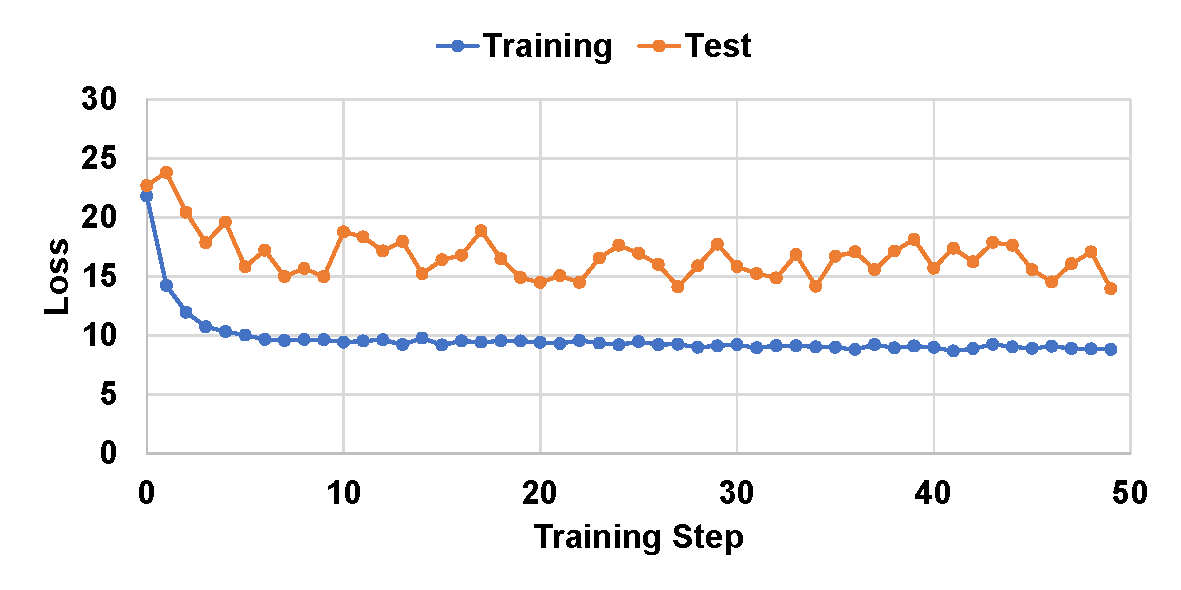
\includegraphics[width=0.48\textwidth]{figs/arrival_loss_3.pdf}
\caption{Loss of arrival time estimation with 3 seismic stations}
\label{fig:arrival_loss_3}
\end{figure}

Figure ~\ref{fig:center_loss_3} shows the loss of location of hypocenter with 3 fast earthquake arrived seismic stations.

\begin{figure}[t]
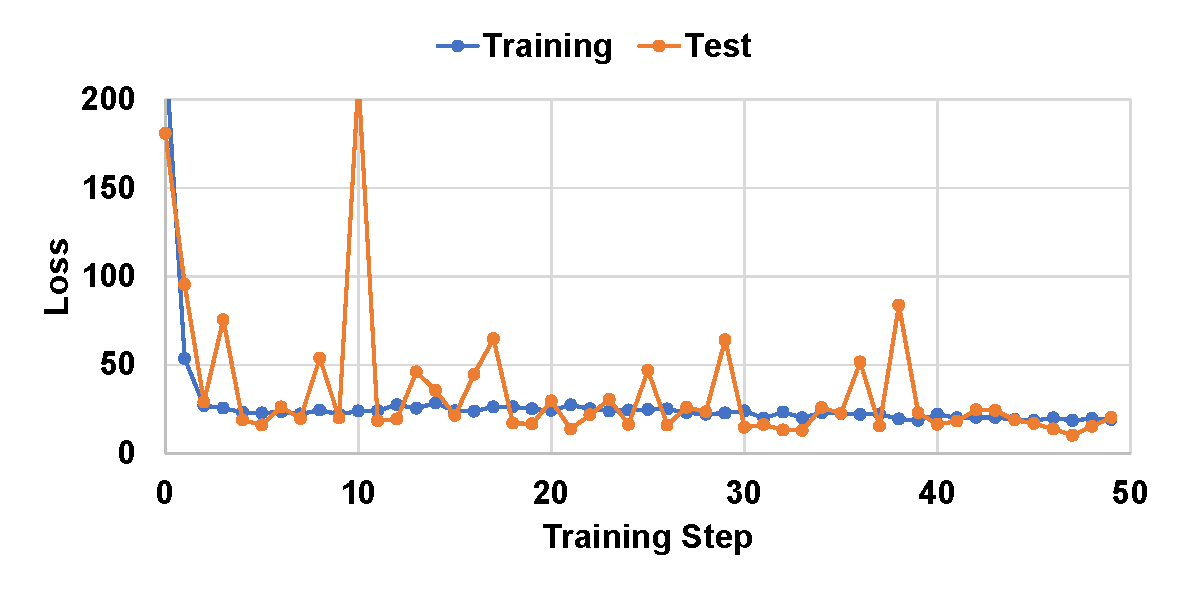
\includegraphics[width=0.48\textwidth]{figs/center_loss_3.pdf}
\caption{Loss of hypocenter estimation with 3 seismic stations}
\label{fig:center_loss_3}
\end{figure}

Figure ~\ref{fig:mag_loss_3} shows the loss of magnitude with 3 fast earthquake arrived seismic stations.

\begin{figure}[t]
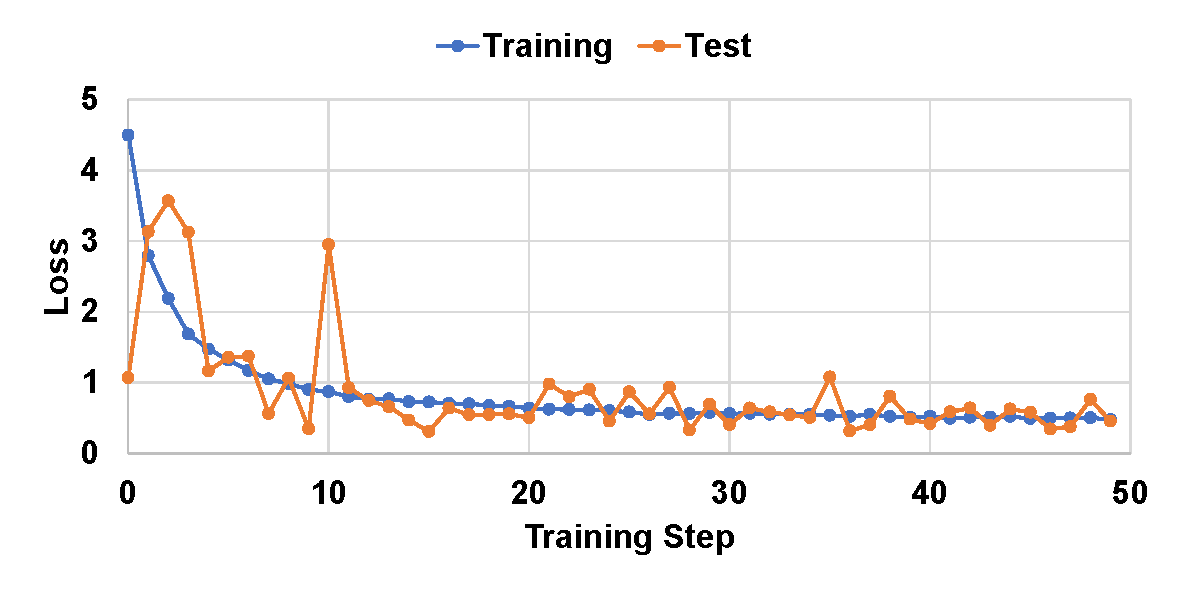
\includegraphics[width=0.48\textwidth]{figs/mag_loss_3.pdf}
\caption{Loss of magnitude prediction with 3 seismic stations}
\label{fig:mag_loss_3}
\end{figure}

%%%

Figure ~\ref{fig:arrival_loss_1} shows the loss of S-wave arrival time with the fastest earthquake arrived seismic stations.

\begin{figure}[t]
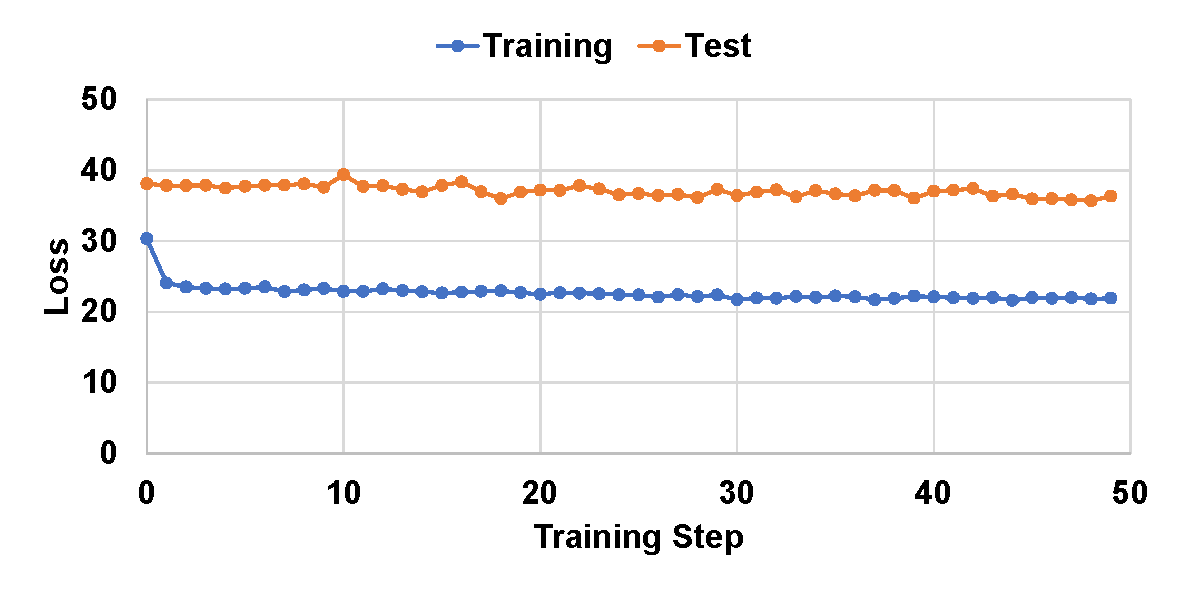
\includegraphics[width=0.48\textwidth]{figs/arrival_loss_1.pdf}
\caption{Loss of arrival time estimation with the fastest seismic stations}
\label{fig:arrival_loss_1}
\end{figure}

Figure ~\ref{fig:center_loss_1} shows the loss of location of hypocenter with the fastest earthquake arrived seismic stations.

\begin{figure}[t]
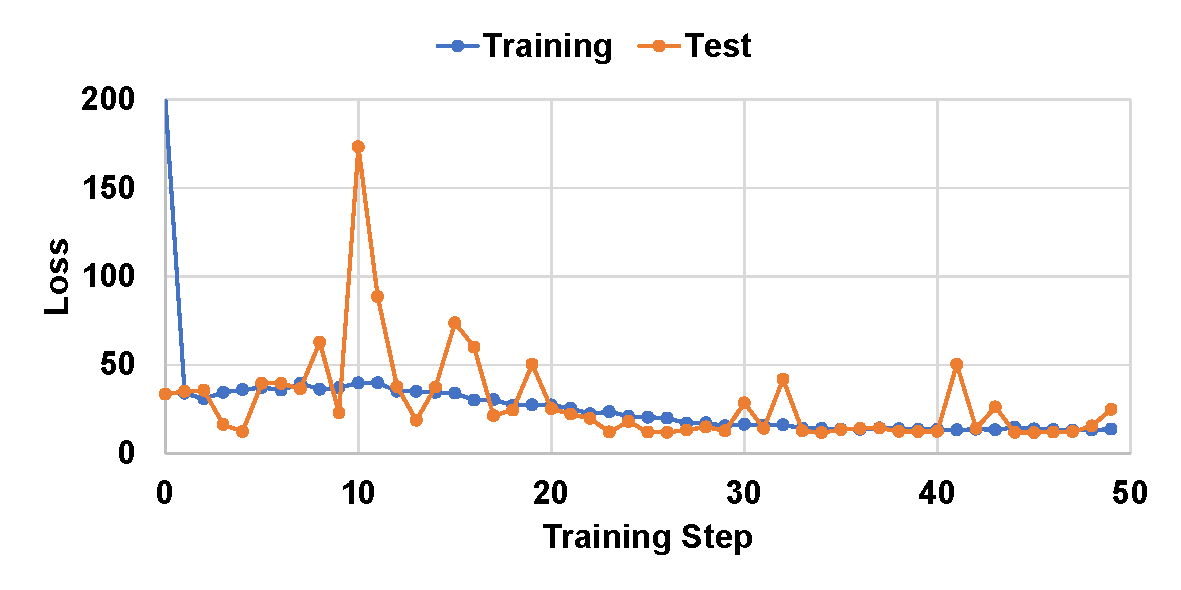
\includegraphics[width=0.48\textwidth]{figs/center_loss_1.pdf}
\caption{Loss of hypocenter estimation with the fastest seismic stations}
\label{fig:center_loss_1}
\end{figure}

Figure ~\ref{fig:mag_loss_1} shows the loss of magnitude with the fastest earthquake arrived seismic stations.

\begin{figure}[t]
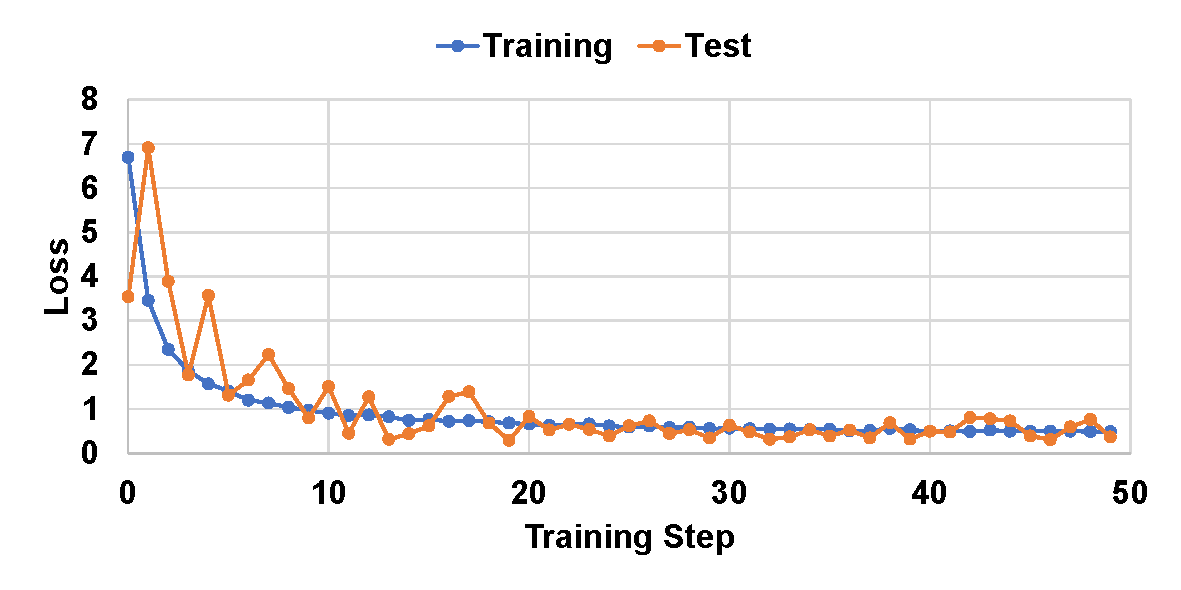
\includegraphics[width=0.48\textwidth]{figs/mag_loss_1.pdf}
\caption{Loss of magnitude prediction with the fastest seismic stations}
\label{fig:mag_loss_1}
\end{figure}

%%%

Figure ~\ref{fig:arrival_each} shows the S-wave arrival time loss of each seismic stations with the 10 fast earthquake arrived seismic stations.

\begin{figure}[t]
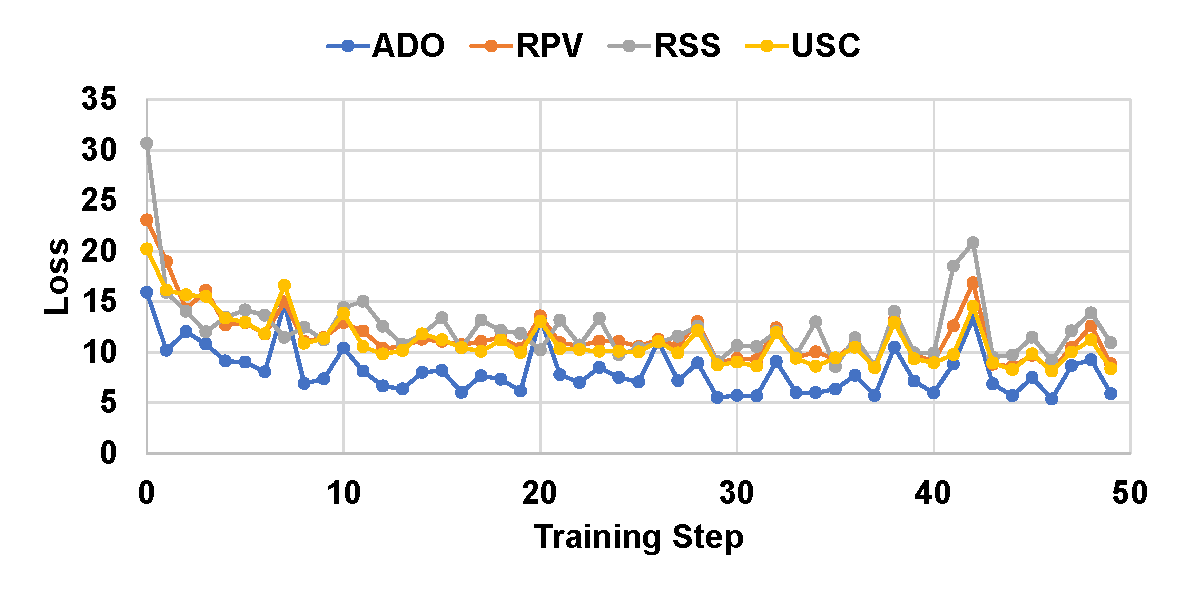
\includegraphics[width=0.48\textwidth]{figs/arrival_loss_detail_10.pdf}
\caption{S-wave arrival time loss of each seismic stations (i.e., ADO, RPV, RSS and USC) with 10 seismic stations}
\label{fig:arrival_each}
\end{figure}

Figure ~\ref{fig:center_each} shows the loss of latitude, longitude and depth with the 10 fast earthquake arrived seismic stations.

\begin{figure}[t]
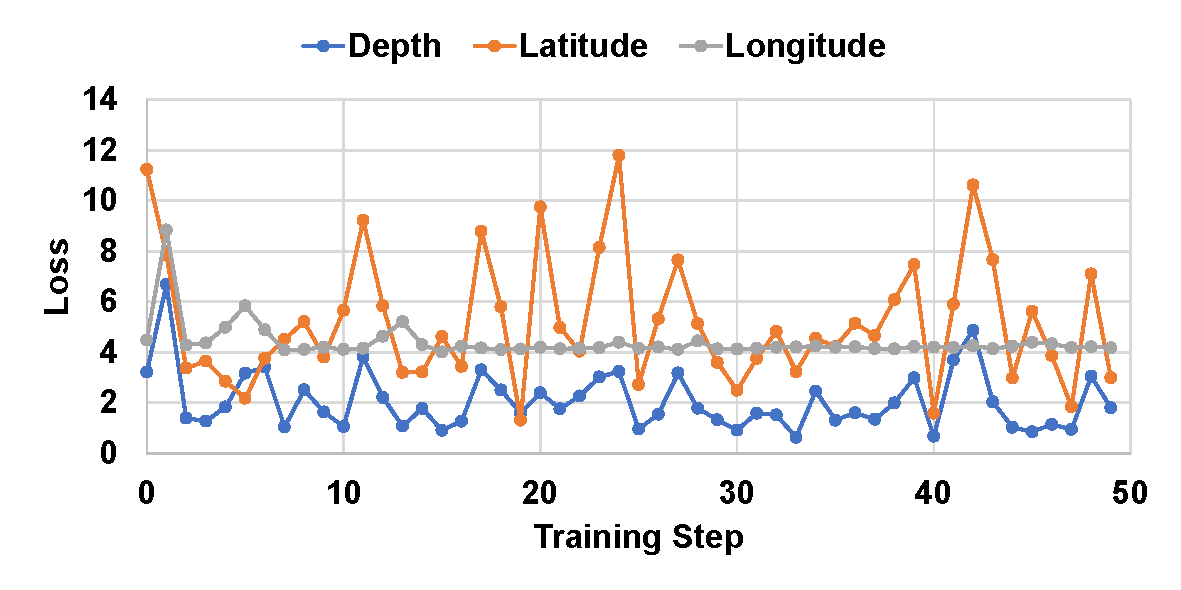
\includegraphics[width=0.48\textwidth]{figs/center_loss_detail_10.pdf}
\caption{latitude, longitude and depth loss with 10 seismic stations}
\label{fig:center_each}
\end{figure}

%%%


\bibliographystyle{ACM-Reference-Format}
\bibliography{refs}

\end{document}
